\documentclass[8pt,a4paper,landscape]{extarticle}
\makeatletter
\def\input@path{{../_shared/}}
\makeatother
\usepackage{cheatsheet}
\usepackage{graphicx}
\usepackage{tikz}
\usetikzlibrary{positioning}

\begin{document}
\begin{multicols*}{4}

\cheattitle{Signal Processing}{}{BA4}

% ============================================================

\section{Basic things}
\begin{defn}[title=Unit impulse | Delta]
$\delta[n] = \begin{cases}1 & n=0\\0 & n\ne 0\end{cases}$, \quad $\delta_m[n] = \delta[n-m]$
\end{defn}

\begin{defn}[title=Unit step]
$u[n] = \begin{cases}1 & n\ge 0\\0 & n<0\end{cases}$
\end{defn}

\begin{defn}[title=Exponential decay]
$x[n] = a^n u[n]$, \quad $0 < a < 1$
\end{defn}

\begin{defn}[title=Sinusoidal oscillation]
$x[n] = A \cos(\omega n + \phi)$, \quad $A\in\R$, $\omega\in\R$, $\phi\in\R$
\end{defn}

\begin{defn}[title=Complex exponential]
$x[n] = A\,e^{j(\omega n + \phi)}$, \quad $A\in\R$, $\omega\in\R$, $\phi\in\R$
\end{defn}

\begin{thm}[title=Energy and Power]
\begin{itemize}
  \item $E_x = \|x\|^2$ \quad (sum or integral of $|x|^2$)
  \item $P_x = \lim_{N\to\infty}\frac{1}{2N+1}\sum_{n=-N}^{N}|x[n]|^2$
  \item $E_x < \infty \;\Rightarrow$ Energy signal ($x \in \ell_2$ or $L_2$)
  \item $P_x < \infty$ and $E_x = \infty \;\Rightarrow$ Power signal
\end{itemize}
\end{thm}

\begin{defn}[title=Time shift by k $\in \Z$]
  $y[n] = \mathcal{S}^{k} x[n] = x[n+k]$
\end{defn}
\begin{defn}[title=Time reversal]
  $y[n] = \mathcal{R} x[n] = \mathcal{S}^{-n} x[0] = x[-n]$
\end{defn}
\begin{thm}[title=Sum of a sequence]
  $\sum_{k=m}^{n} z^{k} = \begin{cases} n-m+1 & z=1 \\ \frac{z^m-z^{n+1}}{1-z} & z\ne 1 \end{cases}$
\end{thm}

% ============================================================

\section{Signal analysis}

\begin{center}
\begin{tikzpicture}[
  font=\tiny, >=stealth,
  node distance=0.42cm and 1.35cm,
  q/.style={align=center, inner sep=1.5pt, text width=1.25cm},
  res/.style={font=\tiny\bfseries\color{blueColor!90!black}},
  yes/.style={->, thick, color=greenColor},
  no/.style={->, thick, color=redColor},
]
  \node[q] (q1) {discr.-time?};
  \node[q, below=of q1] (q2) {finite len.\ $N$?};
  \node[q, below=of q2] (q3) {fin.\ energy\\ $\ell^2(\mathbb{Z})$?};
  \node[q, below=of q3] (q4) {periodic?};
  \node[q, below=of q4] (q5) {power sig.?};
  \node[res, below=0.32cm of q5] (r0) {$\nexists$ FT};

  \node[res, right=of q1] (r1) {Continuous time FT (CTFT)};
  \node[res, right=of q2] (r2) {Discrete FT (DFT)};
  \node[res, right=of q3] (r3) {Discrete time FT (DTFT)};
  \node[res, right=of q4] (r4) {Discrete Fourier Series (DFS)};
  \node[res, right=of q5] (r5) {Generalized DTFT};

  \draw[yes] (q1) -- (q2);
  \draw[no]  (q2) -- (q3);
  \draw[no]  (q3) -- (q4);
  \draw[no]  (q4) -- (q5);
  \draw[no]  (q5) -- (r0);
  \draw[no]  (q1) -- (r1);
  \draw[yes] (q2) -- (r2);
  \draw[yes] (q3) -- (r3);
  \draw[yes] (q4) -- (r4);
  \draw[yes] (q5) -- (r5);
\end{tikzpicture}
\end{center}

\section{DFT: $X[k]$}

\begin{defn}[title=Fourier basis vectors]
$w_k[n] = e^{j\frac{2\pi}{N}kn}$, \quad $n,k=0,\ldots,N-1$.\\
\textbf{Note:} $\mathbf{w}_k = \mathbf{w}_{N-k}^*$.
\end{defn}

\begin{thm}[title=Orthogonality (not orthonormality)]
$\langle \mathbf{w}_h, \mathbf{w}_k \rangle = N\,\delta[h-k]$, where
\[
  \langle \mathbf{x},\mathbf{y}\rangle = \sum_{n=0}^{N-1} x^*[n]\,y[n].
\]
\end{thm}

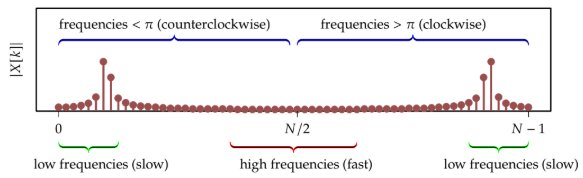
\includegraphics[width=1\linewidth]{images/dft.png}

\begin{prop}[title=DFT matrix form]
$\mathbf{X} = \mathbf{W}\mathbf{x}$, \quad $\mathbf{x} = \tfrac{1}{N}\mathbf{W}^H\mathbf{X}$, where $W_N = e^{-j\frac{2\pi}{N}}$:
\[
  \mathbf{W} =
  \begin{bmatrix}
    W_N^0 & W_N^0 & \cdots & W_N^0 \\
    W_N^0 & W_N^1 & \cdots & W_N^{N-1} \\
    \vdots & & \ddots & \vdots \\
    W_N^0 & W_N^{N-1} & \cdots & W_N^{(N-1)^2}
  \end{bmatrix}
\]
$\mathbf{W}^H\mathbf{W} = N\mathbf{I}$.
\end{prop}

\begin{warn}[title=Powers modulo $N$]
$W_N^n = W_N^{n\,\mathrm{mod}\,N}$ (aliasing property).
\end{warn}

\subsubsection{Small DFT matrices}
\[
  \mathbf{W}_2 = \begin{bmatrix}1&1\\1&-1\end{bmatrix}
\]
\[
  \mathbf{W}_4 = \begin{bmatrix}1&1&1&1\\1&-j&-1&j\\1&-1&1&-1\\1&j&-1&-j\end{bmatrix}
\]

% ============================================================
\section{Properties}
A signal $\mathbf{x}$ is \textbf{symmetric} if $x[n]=x[N-n]$.\\
A signal is \textbf{Hermitian-symmetric} if $x[n]=x^*[N-n]$.

\begin{thm}[title=Symmetry summary]
\renewcommand{\arraystretch}{1}
\begin{tabularx}{\linewidth}{@{}XX@{}}
\toprule
\textbf{Time domain} $x[n]$ & \textbf{Freq.\ domain} $X[k]$ \\
\midrule
Real & $X[-k]=X^*[k]$ \\
Real \& even & Real \& even \\
Real \& odd & Imaginary \& odd \\
Complex \& even & Complex \& even \\
Complex \& odd & Complex \& odd \\
\bottomrule
\end{tabularx}
\end{thm}

% ============================================================
\section{DFS: $X[k]$}
\begin{defn}[title=DFS (Discrete Fourier Series)]
For an $N$-periodic signal $\tilde{x}$:
\[
  \tilde{\mathbf{X}} = \mathrm{DFS}\{\tilde{\mathbf{x}}\} = \mathrm{DFT}\{\tilde{x}[0],\ldots,\tilde{x}[N-1]\}
\]
DFS $\equiv$ DFT: same formulas, different interpretation (explicit periodicity).
\end{defn}

\begin{prop}[title=Circular shift]
$\tilde{x}[n-n_0] \overset{\mathrm{DFS}}{\longleftrightarrow} e^{-j\frac{2\pi}{N}n_0 k}\,\tilde{X}[k]$
\end{prop}

% ============================================================
\section{DTFT: $X(e^{j\omega})$}

\subsection{As a limit of the DFT}
\[
  X[k] \;\longrightarrow\; X(e^{j\omega}) \quad \text{with} \quad \omega = \frac{2\pi k}{N}
\]

\begin{thm}[title=Symmetry summary]
\renewcommand{\arraystretch}{1}
\begin{tabularx}{\linewidth}{@{}XX@{}}
\toprule
\textbf{Time domain} $x[n]$ & \textbf{Freq.\ domain} $X(\omega)$ \\
\midrule
Real & $X(-\omega)=X^*(\omega)$ \\
Real \& even & Real \& even \\
Real \& odd & Imaginary \& odd \\
Complex \& even & Complex \& even \\
Complex \& odd & Complex \& odd \\
\bottomrule
\end{tabularx}
\end{thm}

\subsection{Generalized DTFT (Power Signals)}
Via functionals for infinite-energy signals:
\begin{prop}[title=Constant \& complex exponential]
$\mathrm{DTFT}\{1\}=\delta(\omega)$ \quad (Dirac delta at $\omega=0$)\\
$e^{j\omega_0 n}\overset{\mathrm{DTFT}}{\longleftrightarrow}\delta(\omega-\omega_0)$
\end{prop}
\begin{prop}[title=Sinusoids]
$\cos(\omega_0 n)\overset{\mathrm{DTFT}}{\longleftrightarrow}\tfrac{1}{2}[\delta(\omega-\omega_0)+\delta(\omega+\omega_0)]$\\
$\sin(\omega_0 n)\overset{\mathrm{DTFT}}{\longleftrightarrow}\tfrac{-j}{2}[\delta(\omega-\omega_0)-\delta(\omega+\omega_0)]$
\end{prop}

% ============================================================

\section{FFT}

\begin{prop}[title=Complexity comparison]
\begin{itemize}
  \item Naive DFT: $O(N^2)$ multiplications
  \item FFT: $O(N\log N)$ operations
  \item For $N=10{,}000$: $\sim\!40{,}000$ vs.\ $>100$ million ops
\end{itemize}
\end{prop}

\begin{defn}[title=Decimation in time (Cooley-Tukey)]
Split $N=2^L$ input into even/odd:
$x_e[n]=x[2n]$, $x_o[n]=x[2n+1]$, $n=0,\ldots,\tfrac{N}{2}-1$

Output halves:
$X_a[k]=X[k]$ and $X_b[k]=X[k+\tfrac{N}{2}]$, $k=0,\ldots,\tfrac{N}{2}-1$

\textbf{Butterfly equations:}
\[
  X_a[k] = X_e[k] + e^{j\frac{2\pi}{N}k}\,X_o[k]
\]
\[
  X_b[k] = X_e[k] - e^{j\frac{2\pi}{N}k}\,X_o[k]
\]
where $X_e$, $X_o$ are the $(N/2)$-point DFTs of $x_e$, $x_o$.
\end{defn}

\begin{warn}[title=Cost breakdown]
\begin{itemize}
  \item $2(N/2)^2 = N^2/2$ mults for $\mathbf{X}_e$ and $\mathbf{X}_o$
  \item $N/2$ mults by twiddle factors for $\mathbf{X}_o$
  \item Second half is free (just sign change)
\end{itemize}
Recursion gives $O(N\log_2 N)$ total.
\end{warn}

% ============================================================
\section{Spectrograms (STFT)}

\begin{defn}[title=Short-Time Fourier Transform]
Analyse a signal $\mathbf{x}$ of length $L$ time-locally:
\begin{enumerate}
  \item Slide a window of size $W$ to get $\lfloor L/W \rfloor$ non-overlapping bins
  \item Compute a $W$-point DFT in each bin
  \item Result: 2D time $\times$ frequency representation
\end{enumerate}
\end{defn}

\begin{prop}[title=Kronecker delta in spectrogram]
DFT of a length-$W$ Kronecker delta $\delta[n-m]$ (even shifted): $|X[k]|=1$ for all $k$.\\
$\Rightarrow$ In a spectrogram with window $W$: the bin containing $m$ has \textbf{constant magnitude} $W$ across all frequencies; all other bins are $\mathbf{0}$.
\end{prop}

\begin{warn}[title=Window size trade-off]
\textbf{Large} $W$: good frequency resolution, poor time resolution.\\
\textbf{Small} $W$: good time resolution, poor frequency resolution.\\
This is an instance of the time--frequency concentration duality.
\end{warn}

% ============================================================

\newpage

\section{Filtering I - Digital Filters}

\subsection{LTI Systems}

\begin{defn}[title=Linearity \& time-invariance]
Let $y[n] = \mathcal{H}\{x[n]\}$. \\
\textbf{Linearity} ($\forall\, \alpha,\beta \in\mathbb{C}$, $\forall\, x_1, x_2$):
\[
    \mathcal{H}\{\alpha\, x_1[n] + \beta\, x_2[n]\} \stackrel{?}{=} \alpha\, \mathcal{H}\{x_1[n]\} + \beta\, \mathcal{H}\{x_2[n]\}
\]

\textbf{Time-Invariance} ($\forall\, n_0 \in \mathbb{Z},\ \forall\, x$):
\[
    \underbrace{\mathcal{H}\{x[n - n_0]\}}_{x[\cdot] \,\leftarrow\, x[\cdot - n_0]} \stackrel{?}{=} \underbrace{y[n - n_0]}_{n \,\leftarrow\, n - n_0}
\]
\emph{Key consequence:} an LTI system cannot create new frequency content.

\end{defn}

\subsection{Impulse Response \& Convolution}

\begin{thm}[title=Impulse response]
$\mathbf{h}=\mathcal{H}\boldsymbol{\delta}$. An LTI system is \emph{fully} described by $\mathbf{h}$.
\end{thm}

\begin{defn}[title={Convolution $\mathbf{y}=\mathbf{x}*\mathbf{h}$}]
\[y[n]=\sum_{k=-\infty}^{\infty}x[k]\,h[n-k]\]
\end{defn}

\begin{prop}[title=Convolution properties]
\textbf{Commutativity:} $\mathbf{x}*\mathbf{h}=\mathbf{h}*\mathbf{x}$\\
\textbf{Linearity:} $\mathbf{x}*(\alpha\mathbf{y}+\beta\mathbf{w})=\alpha(\mathbf{x}*\mathbf{y})+\beta(\mathbf{x}*\mathbf{w})$\\
\textbf{Time-shift:} $\mathbf{x}*(\mathcal{S}^k\mathbf{y})=\mathcal{S}^k(\mathbf{x}*\mathbf{y})$\\
\textbf{Associativity:} $(\mathbf{x}*\mathbf{h})*\mathbf{w}=\mathbf{x}*(\mathbf{h}*\mathbf{w})$\\
\textbf{Cascade:} $\mathbf{h}=\mathbf{h}_1*\mathbf{h}_2$; order is irrelevant.
\end{prop}

% --- 3. FILTER PROPERTIES FROM h ---
\subsection{\texorpdfstring{Filter Properties (from $\mathbf{h}$)}{Filter Properties (from h)}}

\begin{defn}[title=FIR vs IIR]
\begin{itemize}
  \item \textbf{FIR} (Finite Impulse Response): $\mathbf{h}$ has finite support. No feedback; \emph{always} BIBO stable.
  \item \textbf{IIR} (Infinite Impulse Response): $\mathbf{h}$ has infinite support. Realizable IIRs use feedback and have a one-sided $\mathbf{h}$.
\end{itemize}
\end{defn}

\begin{defn}[title=Causality]
\begin{itemize}
  \item \textbf{Up to a delay}: $h[n]=0$ for $0>n_0>n$.
  \item \textbf{Anticausal}: $h[n]=0$ for $n>0$; offline use only.
  \item \textbf{Ideal}: $h$ has infinite two-sided support.
\end{itemize}
\end{defn}

\begin{thm}[title=BIBO Stability]
LTI is BIBO stable $\Longleftrightarrow$ $\mathbf{h}$ is absolutely summable:
\[\sum_{k=-\infty}^{\infty}|h[k]|<\infty\]
\end{thm}

\begin{defn}[title=Constant-Coefficient Difference Equation (CCDE)]
\[y[n]=\underbrace{\sum_{k=0}^{M-1}b_k\,x[n-k]}_{\text{feedforward (FIR part)}}-\underbrace{\sum_{k=1}^{N-1}a_k\,y[n-k]}_{\text{feedback (IIR part)}}\]
\textbf{FIR}: all $a_k=0$ for $k\ge 1$.\\
\textbf{IIR}: at least one $a_k\ne 0$ for $k\ge 1$ — recursion introduces a feedback loop.
\end{defn}

% --- 5. FREQUENCY RESPONSE ---
\begin{thm}[title=Frequency Response]
C'est un masque chez les fréquences (ex: lowpass)
\[H(\omega)= \mathrm{DTFT}\{\boldsymbol{h}[n]\} \]
\[\mathcal{H}\{e^{j\omega_0 n}\} = H(\omega_0)\cdot e^{j\omega_0 n}\]
\end{thm}

\begin{thm}[title=Convolution theorem]
\[y=x*h \;\Longleftrightarrow\; Y(\omega)=X(\omega)\cdot H(\omega)\]
\end{thm}

\begin{defn}[title=Filter types by magnitude response]
\begin{itemize}
  \item \textbf{Lowpass}: passes low freqs ($\omega\approx 0$)
  \item \textbf{Highpass}: passes high freqs
  \item \textbf{Bandpass}: passes freqs near $\pm\omega_c$
  \item \textbf{Allpass}: $|H(\omega)|=\text{const}$ — modifies phase only
\end{itemize}
\end{defn}

\subsection{Example of filters}

\begin{defn}[title=Moving Average (MA)]
\[y[n]=\frac{1}{M}\sum_{k=0}^{M-1}x[n-k]\]
$h[n]=\tfrac{1}{M}$ for $0\le n<M$, else $0$.
Causal FIR $\Rightarrow$ always BIBO stable. Big cost.
\end{defn}

\begin{defn}[title=Leaky Integrator (LI)]
\[y[n]=\lambda\,y[n-1]+(1-\lambda)\,x[n], \quad |\lambda|<1\]
\[h[n]=(1-\lambda)\lambda^n\,u[n]\quad\text{(causal, exponential decay)}\]
Causal IIR. Constant cost. Approximates MA of length $M$ with $\lambda=\frac{M-1}{M}$.
\end{defn}

\subsection{Ideal Filters}

\begin{defn}[title=sinc \& rect]
$\mathrm{sinc}(x)=\dfrac{\sin(\pi x)}{\pi x}$,\; $\mathrm{sinc}(0)=1$.\qquad \\
$\mathrm{rect}(x)=\begin{cases}1&|x|\le\tfrac{1}{2}\\0&|x|>\tfrac{1}{2}\end{cases}$

\textbf{DTFT pair}: $\dfrac{\omega_p}{\pi}\,\mathrm{sinc}\!\left(\dfrac{\omega_p}{\pi}n\right)\overset{\mathrm{DTFT}}{\longleftrightarrow}\mathrm{rect}\!\left(\dfrac{\omega}{2\omega_p}\right)$
\end{defn}

\section{Filtering II - Filter Design}
\begin{thm}[title=Modulation theorem]
\[z[n]=x[n]y[n] \;\Longleftrightarrow\; Z(\omega)=X(\omega) * Y(\omega)\]
\end{thm}

\begin{defn}[title=Z-Transform]
\[X(z) = \sum_{n=-\infty}^{\infty} x[n]\,z^{-n}, \quad z\in\mathbb{C}\]
A formal power series in $z^{-1}$; existence requires the sum to converge absolutely for a given $z$.
\end{defn}

\begin{prop}[title=Fundamental properties]
\textbf{Linearity:} $\mathcal{Z}\{\alpha\mathbf{x}+\beta\mathbf{y}\} = \alpha X(z)+\beta Y(z)$\\
\textbf{Time-shift:} $\mathcal{Z}\{x[n-N]\} = z^{-N}X(z)$
\end{prop}

\begin{prop}[title=Link to DTFT]
\[X(e^{j\omega}) = \sum_{n=-\infty}^{\infty} x[n]\,e^{-j\omega n} = \mathrm{DTFT}\{\mathbf{x}\}\]
The DTFT is the z-transform restricted to $|z|=1$
\end{prop}

% --- 2. TRANSFER FUNCTION ---
\subsection{Transfer Function}

\begin{defn}[title=Transfer function $H(z)$]
From $y[n]=h[n]*x[n]$ $\Rightarrow$ $Y(z)=H(z)X(z)$, so $H(z)=\mathcal{Z}\{\mathbf{h}\}=\dfrac{Y(z)}{X(z)}$.\\[4pt]
Applying $\mathcal{Z}\{\cdot\}$ to the CCDE (time-shift: $x[n-k]\to z^{-k}X(z)$):
\[H(z) = \frac{\displaystyle\sum_{k=0}^{M}b_k z^{-k}}{\displaystyle 1+\sum_{k=1}^{N}a_k z^{-k}} = \frac{B(z)}{A(z)}\]
$B(z)$: feedforward (FIR part).\\$A(z)$: feedback (IIR part). FIR: $A(z)=1$.
\end{defn}

\begin{defn}[title=Zeros \& poles — factored form]
\[H(z) = b_0\,\frac{\displaystyle\prod_{k=0}^{M-1}(1-z_k z^{-1})}{\displaystyle\prod_{k=0}^{N-1}(1-p_k z^{-1})}\]
\textbf{Zeros} $z_k$: roots of $B(z)$, where $|H|=0$.\\
\textbf{Poles} $p_k$: roots of $A(z)$, where $|H|\to\infty$.
\end{defn}

% --- 4. STABILITY & ROC ---
\subsection{Stability \& ROC}

\begin{prop}[title=ROC \& causality]
The ROC is the set of $z\in\mathbb{C}$: $\sum_n|x[n]z^{-n}|<\infty$.
Poles bound the ROC — zeros do not affect it.\\[2pt]
\textbf{Causal IIR}: ROC $= \{|z|>R\}$: $R=\max_k|p_k|$.\\
\textbf{FIR}: ROC $= \mathbb{C}$ (except possibly $z=0$).
\end{prop}

\begin{thm}[title=BIBO stability]
Stable $\Longleftrightarrow$ unit circle $|z|=1$ lies inside the ROC\\
$\Longleftrightarrow$ all poles strictly inside the unit circle ($|p_k|<1$).
\end{thm}

\begin{center}
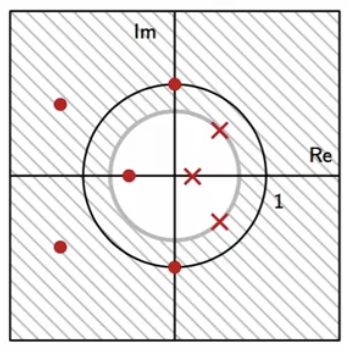
\includegraphics[width=0.47\linewidth]{images/roc_causal_stable.png}\hfill
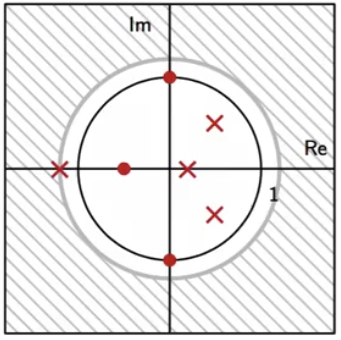
\includegraphics[width=0.47\linewidth]{images/roc_causal_unstable.png}\\[1pt]
{\footnotesize Stable (unit circle in ROC)\hfill Unstable (unit circle not in ROC)}
\end{center}


\subsection{Running Examples in Z-Domain}

\begin{prop}[title=Moving Average — z-domain]
\[H(z)=\frac{1}{N}\cdot\frac{1-z^{-N}}{1-z^{-1}}=\frac{1}{N}\prod_{k=1}^{N-1}(1-e^{j\frac{2\pi}{N}k}z^{-1})\]
$N{-}1$ zeros at $N$-th roots of unity (all except $z=1$); no poles. ROC: all $\mathbb{C}$ except $z=0$. Always stable (FIR).
\end{prop}

\begin{prop}[title=Leaky Integrator — z-domain]
\[H(z)=\frac{1-\lambda}{1-\lambda z^{-1}}, \quad \text{pole at } z=\lambda\]
ROC: $|z|>\lambda$ (causal). Stable $\Leftrightarrow$ $|\lambda|<1$ (pole inside unit circle). As $\lambda\to 1$: pole approaches unit circle, bandwidth narrows.
\end{prop}

\section{Filtering III - Stochastic and Adaptive SP}


\newpage

% ============================================================
\section{Interpolation \& Sampling}

\subsection{The Continuous-Time World}

\begin{defn}[title=CT vs.\ DT paradigm]
\textbf{D:} $x_d[n]\in\ell_2(\mathbb{Z})$, $n\in\mathbb{Z}$, $\omega\in[-\pi,\pi]$, DTFT \newline
\textbf{A:} $x_c(t)\in L_2(\mathbb{R})$, $t$ $\in\mathbb{R}$ [s], \ $f\in\mathbb{R}$ [Hz], CTFT
\end{defn}

\begin{prop}[title=Use cases]
\begin{itemize}
  \item x(t) → $\textbf{[processing]}$ → y(t)
  \item x[n] → $\textbf{[processing for synthesis]}$ → y(t)
  \item x(t) → $\textbf{[processing for analysis]}$ → y[n]
\end{itemize}
\end{prop}

\begin{prop}[title=Real-world frequency]
f = $\#$rep/s = $Hz$ ; $\Omega = 2\pi f$
\end{prop}

\begin{thm}[title=CTFT (more info in cs)]
\begin{itemize}
  \item NOT PERIODIC
  \item NO LIMIT FREQUENCY
\end{itemize}
\end{thm}

\begin{defn}[title=BandLimited (BL) functions]
A CT signal is $F_S$-BL $\Leftrightarrow$ X(f) for $|f|>F_S/2$
\end{defn}

\begin{defn}[title=Support of a function]
The interval where the function is non-trivially zero
\end{defn}

\begin{thm}[title=Sampling theorem (Shannon--Nyquist)]
Any signal $x(t)$ whose highest frequency component is $F_N$ Hz can be sampled with \textbf{no loss of information} using a sampling frequency:
\[F_s \ge 2F_N \quad \left(\text{i.e.\ } T_s \le \tfrac{1}{2F_N}\right)\]
\end{thm}

\subsection{Interpolation x[n] → x(t)}
\begin{prop}[title=Interpolation requirement]
\begin{itemize}
  \item decide on $T_s$ (sampling period)
  \item make sure x(n$T_s$) = x[n]
  \item make sure x(t) is smooth
\end{itemize}
\end{prop}

\begin{prop}[title=Interpolations pros and cons]
\kv{Polynomial}{\textbf{+} $C^\infty$ (max.\ smooth) \ \textbf{--} kernels $L_n^{(N)}$ depend on $N$}\\
\kv{Local}{\textbf{+} kernel indep.\ of $N$ \ \textbf{--} lacks smoothness}
\end{prop}

\begin{thm}[title=Remarkable result]
\[\lim_{N\to\infty} L_n^{(N)}(t) = \mathrm{sinc}(t-n)\]
\end{thm}

\begin{defn}[title=Sinc interpolation]
\[x(t)=\sum_{n\in\Z} x[n]\,\mathrm{sinc}(t-n)\]
$\mathrm{sinc}(m-n)=\delta[m-n]$, $\forall\, m,n\in\Z$\\
\textbf{CTFT pair} ($T_s=1/F_s$)\textbf{:}
\[\varphi(t)=\mathrm{sinc}\!\left(\tfrac{t}{T_s}\right)\longleftrightarrow\Phi(f)=\tfrac{1}{F_s}\,\mathrm{rect}\!\left(\tfrac{f}{F_s}\right)\]
\end{defn}

\begin{defn}[title=Raw Sampling]
\[x[n] = x(nT_s)\]
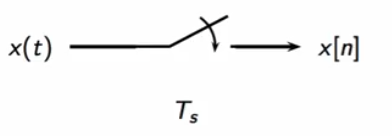
\includegraphics[width=\linewidth]{images/raw_sampling.png}
\end{defn}

\begin{defn}[title=Sinc Sampling]
\[x[n] = \left\langle \mathrm{sinc}\!\left(\frac{t - nT_s}{T_s}\right),\, x(t)\right\rangle\]
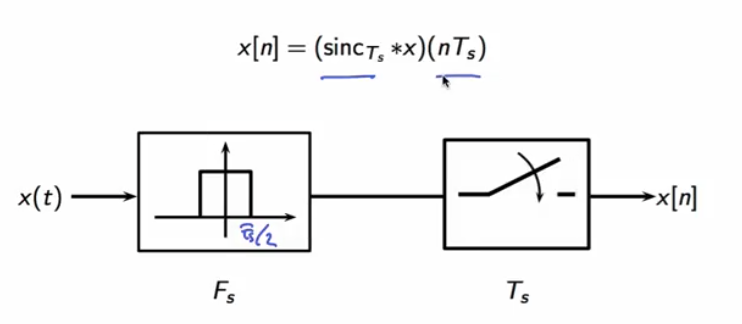
\includegraphics[width=\linewidth]{images/sinc_sampling.png}
\end{defn}

\subsection{Aliasing}
\begin{defn}[title=Sinc Sampling]
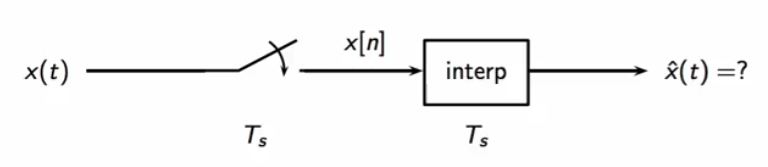
\includegraphics[width=\linewidth]{images/aliasing.png}
Map the frequency into [$-F_s/2$ ; $F_s/2$] to make the signal $F_s$-BL.
\end{defn}


\newpage
% ============================================================
\section{Quick Reference}

\subsection{Geometric sum}
\[
  \sum_{n=0}^{N-1}r^n = \frac{1-r^N}{1-r},\quad r\ne 1
\]
Used in rectangular DFT derivation; also the orthogonality of Fourier vectors (set $r=e^{j\frac{2\pi}{N}(k-h)}$, $k\ne h$).

\subsection{Euler \& trig}
\begin{itemize}

  \item $(e^{j\theta})^* = e^{-j\theta}$
  \item $\cos(a+b)=\cos a\cos b - \sin a\sin b$
  \item $\sin(a+b)=\sin a\cos b + \cos a\sin b$
  \item $\sin a\sin b = \tfrac{1}{2}[\cos(a-b)-\cos(a+b)]$
  \item $\cos a\cos b = \tfrac{1}{2}[\cos(a-b)+\cos(a+b)]$
  \item $\sin a\cos b = \tfrac{1}{2}[\sin(a+b)+\sin(a-b)]$
\end{itemize}

\subsection{Complex number tricks}
\begin{itemize}
  \item $z_1 = z_2^* \Rightarrow |z_1|=|z_2|$ \quad ($|z|=|z^*|$ always)
  \item $z + z^* = 2\,\mathrm{Re}\{z\}$, \quad $z - z^* = 2j\,\mathrm{Im}\{z\}$
  \item $z = z^* \;\Longleftrightarrow\; z\in\mathbb{R} \;\Longleftrightarrow\; \mathrm{Im}\{z\}=0$
  \item $|z_1 z_2| = |z_1||z_2|$, \quad $\angle(z_1 z_2) = \angle z_1 + \angle z_2$
  \item $|z|^2 = z\cdot z^*$
\end{itemize}

\subsection{\texorpdfstring{Inner product in $\mathbb{C}^N$}{Inner product in CN}}
Coefficients: $X[k]=\langle\mathbf{w}_k,\mathbf{x}\rangle$ (projection onto basis).

\subsection{{DTFT inner product in \texorpdfstring{$L_2([-\pi,\pi])$}{L2([-pi,pi])}}}
$\langle\mathbf{F},\mathbf{G}\rangle = \frac{1}{2\pi}\int_{-\pi}^{\pi}F^*(\omega)\,G(\omega)\,d\omega$\\
Set $\{e^{-j\omega n}\}_{n\in\Z}$ forms an orthogonal basis.\\
$x[n] = \langle e^{j\omega n}, X(\omega)\rangle$

\subsection{Key warnings}
\begin{warn}[title=DFT normalization]
\textbf{Analysis}: no $1/N$ factor. \textbf{Synthesis}: $1/N$ factor. Convention: $\mathbf{W}^H\mathbf{W}=N\mathbf{I}$.
\end{warn}

\begin{warn}[title=Phase wrapping]
Phase plots show $\angle X[k] \in [-\pi,\pi]$ (wrapped). Apparent discontinuities are $\pm\pi$ jumps, not real.
\end{warn}

\begin{warn}[title=Real signal DFT]
For real $\mathbf{x}$: $X[k]=X^*[N-k]$. Only first $\lfloor N/2\rfloor+1$ coefficients are independent. Magnitude symmetric around $k=N/2$.
\end{warn}

\begin{warn}[title=Circular vs.\ linear shift]
DFT/DFS time shifts are always \textbf{circular} (modulo $N$). For aperiodic finite signals, multiplying by phase in freq domain gives circular shift.
\end{warn}

\end{multicols*}
\end{document}
